\documentclass[12pt,border=4pt,multi]{article} % \documentclass[tikz,border=4pt,multi]{article}
\usepackage{lingmacros}
\usepackage{tree-dvips}
\usepackage{amssymb} % for mathbb{}
\usepackage[dvipsnames]{xcolor}
\usepackage{forest}
\usepackage{amsmath} % for matrices
\usepackage{xeCJK}
\usepackage{tikz}
\usepackage[arrowdel]{physics}
\usepackage{graphicx}
\usepackage{wrapfig}
\usepackage{listings}
\usepackage{pgfplots, pgfplotstable}
\usepackage{diagbox} % diagonal line in cell
\usepackage[usestackEOL]{stackengine}
\usepackage{multirow}
\graphicspath{{./img}} % specify the graphics path to be relative to the main .tex file, denoting the main .tex file directory as ./
\newcommand\Myperm[2][^n]{\prescript{#1\mkern-2.5mu}{}P_{#2}}
\newcommand\Mycomb[2][^n]{\prescript{#1\mkern-0.5mu}{}C_{#2}}
\definecolor{orchid}{rgb}{0.7, 0.4, 1.1}

\begin{document}

\section*{xl3504\_report\\Xi Liu}
\begin{figure}[h!]
	\centering
	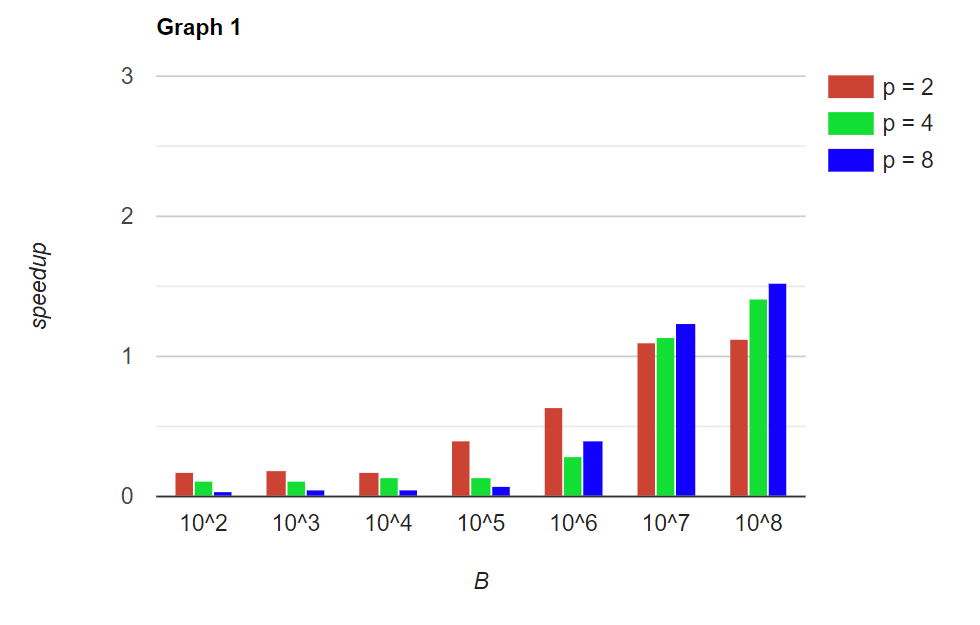
\includegraphics[width=1.1\textwidth, height=0.9\textwidth]{graph1} %img size
\end{figure}
\newpage
\noindent
\begin{figure}[h!]
	\centering
	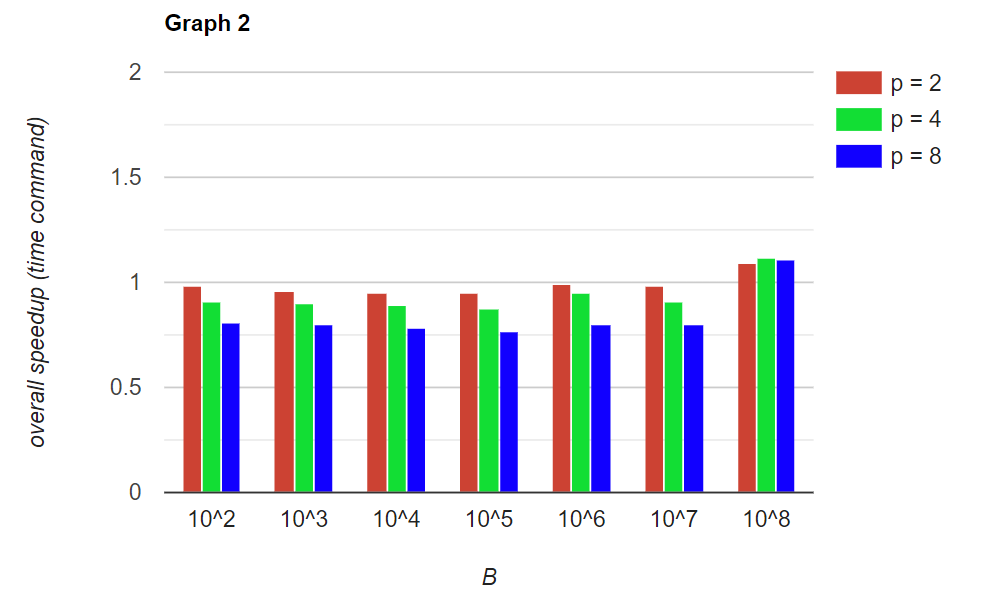
\includegraphics[width=1.1\textwidth, height=0.9\textwidth]{graph2} %img size
\end{figure}\\
\end{document}
